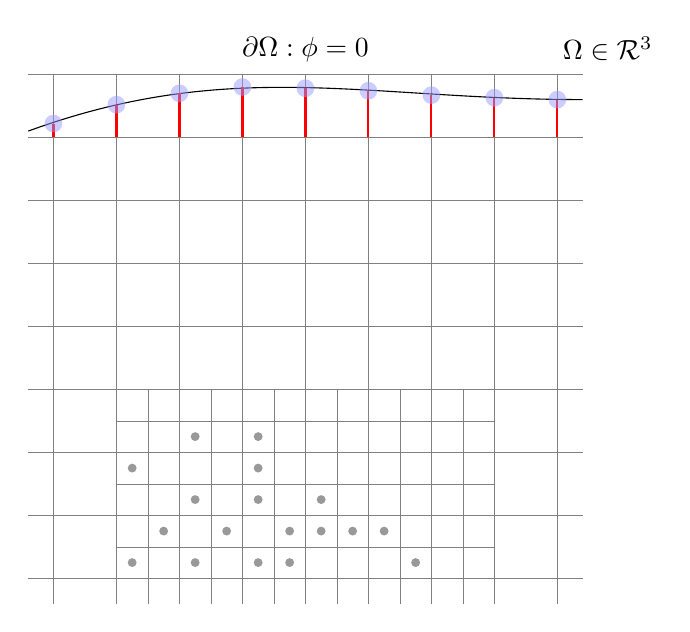
\begin{tikzpicture}[domain=-0.2:4.2,scale=1.6]
    \draw[very thin,color=gray,step=5mm] (-0.2,-0.2) grid (4.2,4);
    \draw[very thin,color=gray,step=2.5mm] (0.5,-0.2) grid (3.5,1.5);
    
    %\filldraw[fill=gray!20,fill opacity=0.8](2,2)--(2,3)--(3,3)--(3,2)--cycle;

    %curved boundart
    \draw (-0.2,3.55) to[out=20,in=180] node [sloped,below] {} (4.2,3.8);
    %\draw (-0.2,3.3) to[out=30,in=180] node [sloped,below] {$\Omega$} (4.2,3.8);
    
    %\coordinate [label=above:\C] (C) at (intersection of B and 1,0--1,1);
    %\fill[black,opacity=.5] C circle (2pt);
  
    %labels
    \node at (4.4,4.2) {$\Omega \in \mathcal{R}^3$};
    \node at (2,4.2) {$\partial \Omega: \phi = 0$};

    %interpolation lines
    \draw[thick,color=red] (0.0,3.5) to (0.0,3.61);
    \draw[thick,color=red] (0.5,3.5) to (0.5,3.76);
    \draw[thick,color=red] (1.0,3.5) to (1.0,3.85);
    \draw[thick,color=red] (1.5,3.5) to (1.5,3.90);
    \draw[thick,color=red] (2.0,3.5) to (2.0,3.89);
    \draw[thick,color=red] (2.5,3.5) to (2.5,3.87);
    \draw[thick,color=red] (3.0,3.5) to (3.0,3.835);
    \draw[thick,color=red] (3.5,3.5) to (3.5,3.815);
    \draw[thick,color=red] (4.0,3.5) to (4.0,3.8);

    %short notice: dont use intersect
    \fill[blue!40,opacity=0.5] (0,3.61) circle (2pt);
    \fill[blue!40,opacity=0.5] (0.5,3.76) circle (2pt);
    \fill[blue!40,opacity=0.5] (1,3.85) circle (2pt);
    \fill[blue!40,opacity=0.5] (1.5,3.9) circle (2pt);
    \fill[blue!40,opacity=0.5] (2,3.89) circle (2pt);
    \fill[blue!40,opacity=0.5] (2.5,3.87) circle (2pt);
    \fill[blue!40,opacity=0.5] (3,3.835) circle (2pt);
    \fill[blue!40,opacity=0.5] (3.5,3.815) circle (2pt);
    \fill[blue!40,opacity=0.5] (4,3.8) circle (2pt);

    %particles
    \fill[black!40] (0.625,0.125) circle (1pt);
    \fill[black!40] (0.625,0.875) circle (1pt);
    
    \fill[black!40] (0.875,0.375) circle (1pt);

    \fill[black!40] (1.625,1.125) circle (1pt);
    
    \fill[black!40] (1.375,0.375) circle (1pt);

    \fill[black!40] (1.125,1.125) circle (1pt);
    \fill[black!40] (1.125,0.625) circle (1pt);
    \fill[black!40] (1.125,0.125) circle (1pt);
    
    \fill[black!40] (1.625,0.875) circle (1pt);
    \fill[black!40] (1.625,0.125) circle (1pt);
    \fill[black!40] (1.625,0.625) circle (1pt);

    \fill[black!40] (1.875,0.375) circle (1pt);
    \fill[black!40] (1.875,0.125) circle (1pt);
    
    \fill[black!40] (2.125,0.375) circle (1pt);
    \fill[black!40] (2.125,0.625) circle (1pt);

    \fill[black!40] (2.375,0.375) circle (1pt);

    \fill[black!40] (2.625,0.375) circle (1pt);
    
    \fill[black!40] (2.875,0.125) circle (1pt);

\end{tikzpicture}
